%% APPENDIX A -- spectral response, frequency conventions, primary-beam response.
%% Owner: appendix-triage.  Carries \label{app:conventions} (cited by
%% 04_method.tex) and \label{app:pbresp}.
\section{Spectral response, frequency conventions and the primary-beam
response}
\label{app:conventions}

Checking a threshold in this paper needs three things: the frame every
frequency is quoted in, the instrumental response that separates a channel
threshold from a transmitter power, and the primary-beam factor that turns a
measured noise into a flux at the star. The per-window catalogue,
\texttt{catalogue/windows.csv} in the deposit, carries the columns each of
them uses.


\begin{figure}
\centering
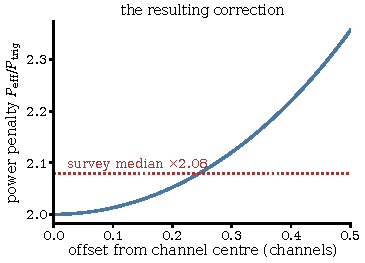
\includegraphics[width=\columnwidth]{figures/hanning_response.pdf}
\caption{Why the nominal channel threshold is not the transmitter
threshold. ALMA applies online Hanning smoothing by default, so an
intrinsically unresolved carrier is spread over neighbouring channels and
the peak channel holds only part of its power: half at a channel centre,
\HanWorst{} on a boundary. The threshold is set in units of the channel
noise, so the power a transmitter must radiate to reach it is larger than
the nominal figure by the reciprocal of that fraction, plotted here against
where in the channel the carrier falls. This is the whole of the difference
between $P_{\rm trig}$ and $P_{\rm eff}$.}
\label{fig:hanning}
\end{figure}

\subsection{Frequency frames, linewidth and smearing}
%% (subsection label retired: nothing cites it)

Every frequency axis here --- searched spectra, tabulated ranges and
crossing frequencies alike --- is \emph{topocentric} as delivered by the
ALMA correlator, and the search itself applies no velocity-frame shift.
Velocities enter at the vetting stage, where the line mask is evaluated in
each star's own rest frame: it carries every crossing frequency to the
barycentre at its own block's epoch and then to the stellar frame before
comparing it with a transition (Appendix~\ref{app:linemask}). The residual
error is then the catalogue radial-velocity uncertainty alone, a few
km\,s$^{-1}$ within 40\,pc; second-order relativistic terms at the
\MaskHalfKms\,km\,s$^{-1}$
scale are $\lesssim5$\,kHz at 350\,GHz, below the finest native channel
searched. The stacking is drift-aligned and inverse-variance weighted:
coherent in frequency trajectory, not in electric-field phase.

The native channel width is also the linewidth convention for every EIRP
threshold. The statistic is the single-channel flux density after drift
correction, so EIRP$_{\rm trig}$ is the minimum \emph{total} power of a
channel-confined carrier, flat in the assumed linewidth below the channel and
never a spectral power density; flatness is exact only for a centred tone,
and a boundary-straddling one divides its power between two channels, which
is the loss the injections carry and one reason EIRP values are quoted to two
significant figures. The Hz-resolution
surveys' limits are total powers in the same sense, each the best case of
its own channelisation, which makes the axes of Fig.~\ref{fig:context}(a)
commensurable. One number fixes the scale, illustratively and not
achievably: rechannelising the median Class~A window's
\SqrtScaleChanKHz\,kHz to the \SETIChanHz\,Hz of a dedicated narrowband
search would divide the threshold by $\SqrtScaleFac$, and no reprocessing
recovers resolution the correlator never recorded.

Channel widths come from the measurement sets' own CHAN\_WIDTH; MS~v2
defines no ``EFFECTIVE\_BANDWIDTH'' column, so the quoted channelisations are
separations and are not claimed to be noise bandwidths.

ALMA applies online Hanning smoothing by default \citep{ALMAHandbook}, so
the spectral response is ${\sim}2$ channels wide and neighbouring channels are correlated
(Fig.~\ref{fig:hanning}). For the $0.25/0.5/0.25$ kernel the coefficients
are $\rho_1=\HanRhoOneFrac=\HanRhoOne$ and $\rho_2=\HanRhoTwo$, with
$\sigma_{\rm smoothed}/\sigma_{\rm raw}=\HanSigRatio$: the correlation is
not confined to adjacent channels, the lag-two term being a sixth. The
peak-channel fractions \HanWorst--\HanBest, median \HanMed, and the
resulting $\times\HanFacBest$--$\times\HanFacWorst$ optimism of a nominal
threshold are given in \S\ref{sec:method}; the released catalogue carries the
nominal threshold and both corrected values for every window.

\emph{The injected carriers are deposited with the correlator's own channel
response, at a sub-channel phase drawn afresh for each tone, so the smoothing
loss sits inside the measured completeness rather than being applied to it.}
The deposited profile is the tone divided between the two channels it
straddles and then passed through the three-point kernel, which leaves
\InjDepCentre{} of the flux in the peak channel for a carrier at a channel
centre and \InjDepEdge{} for one on a boundary, against \InjRespEdge{} for
the exact transform of the lag window; averaged over phase the deposition
therefore falls \InjShortPct{} per cent short of the ideal response, and the
completeness is conservative by that much. Where in a channel a carrier was
placed makes no difference to its recovered signal-to-noise: the medians over
\InjNPhaseTone{} tones agree across the whole range of sub-channel phase to
\InjPhaseFlatPct{} per cent, because a carrier at a typical searched drift
rate crosses about \InjDriftChan{} channels during one observation and so
samples the whole response. Since the loss is carried end to end it must not
be applied to the result as well: at the ninety per cent point of the
recovery curve the peak channel holds $\InjPeakAtNinety\times$ the nominal
trigger flux, which is that factor of about two, already spent.

Two measurements fix the smoothing state. The retained per-integration
residuals of the second-stage local null have a lag-one spectral
autocorrelation of \LNLagOne{} against the Hanning prediction \HanRhoOne, so
the correlation is instrumental and those spectra are smoothed and
un-averaged; and the archive's reported effective spectral resolution is
exactly twice the channel separation in \NHanTwo{} of the \NHanKnown{}
windows, in both correlator modes. The other \NHanOther{} report a smaller
ratio, the signature of online channel averaging, where the peak-channel loss
is smaller; every released window has a reported resolution, so the blanket
factor is right for the great majority of both classes. \emph{The correlation model is truncated at
lag two}: the baseline step, a per-integration median over up to \MedWin{}
channels, could imprint longer-range correlation that the released products
retain no residuals to measure, which would make the independent-trials count
of Appendix~\ref{app:falsealarm} an over-estimate.

\emph{Transmitters wider than one channel.} The baseline filter
(\S\ref{sec:statistic}) is flat for features narrower than roughly half its
effective width $W$ and falls to zero above $W$, so the survey's sensitivity
is to channel-confined morphologies and $W$ is the linewidth ceiling:
\MedWinFineLo--\MedWinFineHi{} channels over the fine class and
\MedWinCoarseLo--\MedWinCoarseHi{} over the coarse one, that is
${\approx}\MedWinCeilFineMHz$\,MHz at \ChanFineKHz\,kHz and
${\approx}\MedWinCeilCoarseGHz$\,GHz at \ChanCoarseMHz\,MHz. Within that
ceiling a top-hat transmitter spanning $N_{\rm ch}$ native channels has
per-channel flux the total divided by $N_{\rm ch}$ at unchanged noise, so
its threshold is $N_{\rm ch}$ times the single-channel one, which is the
rescaling the main text applies to signals broader than one channel.

\emph{Intra-integration smearing.} A drift smeared by $\Delta$ channels within
one integration keeps $\eta_{\rm smear}=\mathrm{sinc}(\pi\Delta/2)$ of the peak
amplitude, so the effective threshold is
$\mathrm{EIRP}_{\rm trig}/\eta_{\rm smear}$. The excursion can be evaluated
wherever the release carries the integration count, which is \CsNDumpWin{} of
the \NWindows{} windows; over those it reaches at most 1.10 channels. Only
\NSmearLo{} of them have $\eta_{\rm smear}<0.99$ --- \SmearList{} --- and the
other \NSmearOk{} agree with their nominal thresholds to better than one per
cent. Compounding
the worst smearing penalty with the worst Hanning factor gives
$\times\CompoundWorst$ for those few, a product no released column carries.

\subsection{The primary-beam response, and the two columns that let a reader
recompute it}
%% (subsection label retired: nothing cites it)

The sensitivity quoted for a window is $S_{\min}=5\sigma/A$, where $A$ is the
primary-beam response at the star's offset from the phase centre: the noise
$\sigma$ is measured in apparent flux, the limit is quoted in true flux, and
the two differ by $A$. That offset is not a nuisance. Archival fields are
pointed at a catalogue position, often decades old, while these are
high-proper-motion stars, so the star can sit well off axis: over the
\PbNWin{} released windows the offset has a median of \PbOffMed$''$, a 99th
percentile of \PbOffPNN$''$ and a maximum of \PbOffMax$''$, and $A$ runs from
\PbAMed{} in the median down to \PbAMin, below $0.99$ on \PbNLowNN{} windows
and below $0.9$ on \PbNLowN. \emph{None} falls below one half, and every one
of the low-response windows is a physically explicable J2000 pointing on a
fast-moving star rather than an error. A window is kept only where the
response is at least \PbFloorResp, a correction of at most
$\times\PbFloorCorr$, since at low response a small error in the beam model
becomes a large error in inferred flux. The offsets are bimodal and the floor
sits in the gap: the last retained window has response \PbGapKeptResp{} at
$\PbGapKeptU\,\theta_{\rm PB}$, the first window beyond it \PbGapHeldResp{}
at $\PbGapHeldU\,\theta_{\rm PB}$, and nothing lies between, so the rule
binds prospectively and excludes none of the \NWindows{} released windows.
Beyond it lie the \EpsEriNWin{} $\epsilon$\,Eri Band~6 windows, also past the
first sidelobe transition where the Gaussian form fails. They are
\emph{withheld}, enter no number here and are absent from the released
catalogue.

\emph{The correction is applied exactly once.} The offset is computed for
every measurement set from its own \texttt{FIELD::PHASE\_DIR} and the
propagated stellar position, so no window carries a zero-by-assumption
offset, and it enters in one place only: $S_{\min}=5\sigma/A$ closes on all
\PbSminClosed{} released rows to \PbSminWorstRes{} in relative terms. The
count is in two parts, because on \PbSminTaut{} rows whose products are not
retained $A$ is back-solved from $5\sigma/S_{\min}$ and flagged as such, so
there the closure is arithmetic; the audit is a test on the other
\PbSminIndep{} rows, where $A$ comes from the search's own stored geometry and
closes to \PbSminIndepRes. Nothing else needs correcting: the statistic of
Eq.~\ref{eq:tstar}, the control ranks and the attribution are \emph{ratios}
formed inside one window, in which $A$ divides out identically.

\emph{Three columns carry the geometry, and which is which matters.}
\texttt{pb\_offset\_arcsec} is the offset. \texttt{pb\_atten} is the response
applied: a Gaussian of full width $\RingPbCoefCode\,\lambda/D$ --- an Airy
first-null coefficient --- evaluated \emph{at each window's own dish
diameter}, which is reproduced over all \NWindows{} released rows to
$\SensPbResid$, while the same Gaussian forced to $D=12$\,m for every row
departs from the column by up to $\SensPbResidTwelve$. The third,
\texttt{theta\_pb\_arcsec}, \emph{is} $\RingPbCoefCode\,\lambda/D$ at
$D=12$\,m for every window, including the \PbNAcaRow{} taken on the
\PbAcaRatio$\times$ smaller compact-array dishes, so $A$ cannot be recomputed
from it and \texttt{pb\_atten} has to be read instead.

\emph{The beamwidth convention is a bounded systematic, and the release
carries both conventions so that a reader need not take ours.} ALMA's
primary-beam full width is $\RingPbCoef\,\lambda/D$, narrower than the
first-null coefficient, so it attenuates more and makes every limit
\emph{shallower}: by nothing at all in the median window, by more than one
per cent in \SensPbNOnePct{} of \NWindows{} and by more than ten in
\SensPbNTenPct, the largest being $+\SensPbShiftMaxPct$ per cent --- those
few all \SensPbWorstStar{} at \SensPbWorstOff$''$ off axis. The lowest
response in the release moves \SensPbAMin{} to \SensPbAMinAlma, still clear
of the \SensPbFloor{} retention floor but by a margin small enough to be
worth saying. \texttt{pb\_atten\_fwhm} in the deposit carries that column
window by window, with each window's own $\theta_{\rm PB}$ beside it.
Changing the convention changes no disposition, because $A$ divides out of
every ratio formed inside a window, and the published identity
$S_{\min}=5\sigma/A$ is left closing on the response that formed it. The
remaining model uncertainty is also bounded by measurement: CASA's
blocked-Airy response is better physics than either Gaussian, the largest
ratio to it over the whole release is \PbModelMax, and the counts of systems
reaching $10^{15}$\,W are identical under any of the three.

\emph{The star's apparent direction includes the annual parallax, and the
amplitude a compact source retains when that is left out of the assumed phase
centre is measured rather than modelled.} The displacement decides whether the
loss can be treated as a scalar at all: a small fraction of a synthesised beam
attenuates a compact source and does nothing else, while a displacement
approaching a beam puts the phase wrong on the longest baselines. Re-extracting
the \SensNReextWin{} windows of \SensNReextBlock{} blocks furthest out at the
full apparent position --- proper motion, parallax, and radial velocity where
catalogued --- leaves each window's own noise unchanged to
\SensReextNoiseMaxPct{} per cent and alters no disposition, but it cannot test
the amplitude factor, \emph{because the factor describes a source and those
windows hold none}. The statistic at the star is a maximum over a plane of
drift trajectories, so moving the extraction point by two thirds of a beam
draws a nearly independent noise realisation: the ratio scatters from
\SensReTstarLo{} to \SensReTstarHi{} about a median of \SensReTstarMed,
nowhere near the \SensPxLargePred{} the model predicts for a source. So a
source was put there. A carrier injected at the apparent position and recovered
from the \emph{same} visibilities at both positions returns a ratio that
\emph{is} the normalised dirty beam at the omitted displacement, measured on
that block's own baselines with no model in it
(Table~\ref{tab:pxmeasured}). That it exceeds the model at the larger
displacement is the search's doing: maximising over a plane of trajectories
lets a partly decohered carrier still find a cell, so the pipeline retains more
than the beam amplitude alone and a limit corrected by the model is shallower
than it needs to be.

\begin{table}
\centering
\caption{\textbf{The amplitude retained at a mis-assumed stellar position,
measured.} A carrier injected at the star's apparent position and recovered
from the same visibilities twice: once with the extraction phase-rotated to
that position, once to the parallax-free one. The ratio of recovered
signal-to-noise is the normalised dirty beam at the omitted displacement; the
prediction is the model each window's own correction uses.}
\label{tab:pxmeasured}
\footnotesize
% GENERATED by sens_r11.py -- do not hand-edit.
\begin{tabular}{@{}l@{~~}r@{~~}r@{~~}r@{~~}r@{}}
\hline
star & offset & predicted & measured & tones \\
 & (beams) & & & \\
\hline
$\tau$~Cet & 0.25 & 0.889 & $0.920^{+0.017}_{-0.014}$ & 12 \\
$\gamma$~Lep & 0.67 & 0.485 & $0.583^{+0.027}_{-0.044}$ & 12 \\
\hline
\end{tabular}

\end{table}

\emph{The injection campaign is blind to $A$ by construction, and the bias
that follows is exactly zero.} The injector deposits an unattenuated amplitude
at the star's own direction cosines, and on all \PbInjNUnit{} scored units
the ladder is referred to the \emph{apparent} $5\sigma$: an injected apparent
amplitude recovered nine times in ten implies a true flux larger by $1/A$
while $P_{\rm trig}$ is the power of a true $5\sigma/A$, so $A$ cancels
identically. The cancellation is tested and not vacuous --- \PbInjNDistinct{}
of the \PbInjNUnit{} units have apparent and corrected $S_{\min}$ differing by
more than a part in a thousand. Being self-consistent in apparent flux, the
campaign cannot falsify the beam model; and injected configurations reach only
$A\ge\PbInjAMin$, whereas \PbNBeyond{} windows on \PbNBeyondStar{} stars lie
further off axis, down to $A=\PbBeyondAMin$, so a limit quoted for one of
those rests on an extrapolated curve. Their \PbNBeyondCross{} crossings are
ratios and unaffected.

\emph{Four rows carry a catalogued noise that no retained product
reproduces}, and they are declared rather than reconciled: \PbGapN{} windows
of \PbGapStar{} in block \texttt{\PbGapEb}, whose catalogued $\sigma$ is
\PbGapPctLo--\PbGapPctHi{} per cent \emph{higher} than the surviving
product's, so the limits there are weaker and not stronger. With the
\PbGapNoProd{} windows whose products are not retained at all, the declared
provenance gap is \PbGapDeclared{} windows; the attenuation columns are
unaffected, $A$ coming from a retained product at the same position where
$A\ge\PbGapAMin$.

%% ------------------------------------------------------------------
%% REQUEST (appendix-triage -> integrator / 08_backmatter owner):
%%   \label{app:repro} no longer exists.  08_backmatter.tex cites it in the
%%   Data Availability statement.  Repoint that sentence at
%%   \ref{app:conventions}, or better, drop the cross-reference and name the
%%   deposit directly -- the sentence is about the release, not an appendix.
%% REQUEST (appendix-triage -> numbers):
%%   The UV Ceti worked example (flux -> EIRP) was deleted from this appendix
%%   because two of its four numbers are typed literals with no macro
%%   (1.21e-29 W/m2/Hz and 1.6e13 W).  If a worked example is wanted back,
%%   three macros are needed: the flux density, the implied EIRP and the
%%   distance used.  It is the clearest single verification aid in the paper.
%% REQUEST (appendix-triage -> stack-discussion, Section 6):
%%   The transmitter-power benchmark was deleted here.  Exactly one benchmark
%%   should survive, in Section 6: a \BenchDiam-m aperture radiating 1 MW at
%%   230 GHz, aperture efficiency 0.7, giving EIRP \BenchEirpSeven W, which
%%   the median Class A effective threshold \PeffWinMedA W misses by a factor
%%   \BenchEffRatio.  Macros \BenchDiam, \BenchGainSeven, \BenchEirpSeven,
%%   \BenchEffRatio, \PeffWinMedA and equation eq:gain are otherwise
%%   unreferenced and will be retired.  The Arecibo scale and the
%%   frequency-scaled Arecibo figure are deliberately not carried forward.
%% ------------------------------------------------------------------

%% ★ tab:blockledger MOVED HERE from Sec. 3 in the v4.12 length pass.  It is a
%% full-width table* worth 0.53 pp of the main text; Sec. 3.1 now carries its
%% headline rows in prose and cites it, which is what R2-M2(a) asked for.
\begin{table*}
\centering
\scriptsize
\caption{The block and window ledger. Every set of execution blocks used
anywhere in this paper, with the results it enters; the rows sum, and each
indented group sums to the row above it. The primary census is the survey:
unless a statement names one of the other sets, it is computed over that row.
Hours are on-source hours. Confirmed planet counts, here and in the deposited
target list, are taken from the \SfHostCatalogue{} \SfHostTable{} table
\citep{NEA2013}, accessed \SfHostDate.}
\label{tab:blockledger}
%% GENERATED by blockledger_v411.py -- do not hand-edit.
\begin{tabular}{@{}p{0.285\textwidth}rrrrrp{0.275\textwidth}@{}}
\hline
Set of execution blocks & Blocks & Windows & Stars & Systems & Hours & Results it enters \\
\hline
Archival scope: blocks the query exposes & 656 & -- & -- & -- & -- & defines the scope; the sum of the next two rows \\
\hspace{1.1em}\ldots{} processed with the frozen pipeline & 479 & -- & -- & -- & -- & the second panel below \\
\hspace{1.1em}\ldots{} not processed at the freeze & 177 & -- & -- & -- & -- & the third panel below \\
\hline
Processed with the frozen pipeline$^{c}$ & 484 & -- & -- & -- & -- & the sum of the three rows below \\
\hspace{1.1em}\textbf{Primary census} & 404 & 1651 & 89 & 82 & 1094 & every limit, the crossing list, every chance expectation \\
\hspace{2.2em}Class~A, fine channels$^{a}$ & -- & 402 & 65 & 60 & 227 & the drifting-carrier experiment \\
\hspace{2.2em}Class~B, coarse channels$^{a}$ & -- & 1249 & 88 & 81 & 867 & the spectral-excess experiment \\
\hspace{1.1em}Reserved hold-out & 77 & 315 & 36 & -- & 214 & the rank displacement, the false-alarm tail factor, the radial control profile \\
\hspace{1.1em}No window survived the quality cut & 3 & 0 & 0 & 0 & 0 & nothing \\
\hline
Not processed at the freeze: what became of each & 177 & -- & -- & -- & -- & the sum of the five fates below \\
\hspace{1.1em}Calibrated and searched & 144 & -- & -- & -- & -- & the sum of the four rows below \\
\hspace{2.2em}\textbf{Archival extension}, reported & 115 & 463 & 16 & 16 & 269 & recurrence, and the null on data the frozen pipeline had not seen \\
\hspace{2.2em}Searched after the extension was frozen & 8 & 32 & -- & -- & -- & nothing; later than the reported extension \\
\hspace{2.2em}Withheld: primary-beam form invalid$^{d}$ & 8 & 32 & -- & -- & -- & nothing; withheld \\
\hspace{2.2em}No window reached the export & 13 & 0 & -- & -- & -- & nothing \\
\hspace{1.1em}No calibration in the ALMA delivery & 18 & -- & -- & -- & -- & nothing; the archival gap \\
\hspace{1.1em}Calibration failed & 11 & -- & -- & -- & -- & nothing; the archival gap \\
\hspace{1.1em}Not attempted & 3 & -- & -- & -- & -- & nothing; the archival gap \\
\hspace{1.1em}Working disk insufficient & 1 & -- & -- & -- & -- & nothing; the archival gap \\
\hline
Beyond 40\,pc: out-of-sample control & 47 & 198 & 22 & -- & 88 & the external null; no science count \\
External calibration sample$^{b}$ & 326 & 1322 & 56 & -- & -- & the rank calibration and the positive control; no science count \\
\hline
\end{tabular}

{\footnotesize $^{a}$The two classes partition the census windows, not its blocks: 252 blocks carry a Class~A window and 389 a Class~B one, and most carry both.\\ $^{b}$Not a subset of the archival scope: it includes blocks toward stars outside the 40\,pc work list, so its blocks cannot be placed inside this ledger.\\ $^{c}$This panel and the scope panel above overlap rather than add: 479 of these 484 blocks are the in-scope row above, and the other 5 carry no member observing unit in the archive metadata, so the scope query does not expose them. 3 of the 5 are in the primary census.\\ $^{d}$Every one is an $\epsilon$\,Eri Band~6 block, where the Gaussian primary-beam form is not valid; the same rule withholds 12 windows from the primary census.}

\end{table*}

